\documentclass{article}
\usepackage[a4paper, portrait, margin=1.1811in]{geometry}
\usepackage[english]{babel}
\usepackage[utf8]{inputenc}
\usepackage[T1]{fontenc}
\usepackage{helvet}
\usepackage{etoolbox}
\usepackage{graphicx}
\usepackage{titlesec}
\usepackage{caption}
\usepackage{booktabs}
\usepackage{xcolor} 
\usepackage[colorlinks, citecolor=cyan]{hyperref}
\usepackage{caption}
\captionsetup[figure]{name=Figure}
\graphicspath{ {./images/} }
\usepackage{scrextend}
\usepackage{fancyhdr}
\usepackage{graphicx}
\newcounter{lemma}
\newtheorem{lemma}{Lemma}
\newcounter{theorem}
\newtheorem{theorem}{Theorem}

\fancypagestyle{plain}{
	\fancyhf{}
	\renewcommand{\headrulewidth}{0pt}
	\renewcommand{\familydefault}{\sfdefault}
}

%\pagestyle{plain}
\makeatletter
\patchcmd{\@maketitle}{\LARGE \@title}{\fontsize{16}{19.2}\selectfont\@title}{}{}
\makeatother

\usepackage{authblk}
\renewcommand\Authfont{\fontsize{10}{10.8}\selectfont}
\renewcommand\Affilfont{\fontsize{10}{10.8}\selectfont}
\renewcommand*{\Authsep}{, }
\renewcommand*{\Authand}{, }
\renewcommand*{\Authands}{, }
\setlength{\affilsep}{2em}  
\newsavebox\affbox
\author{\textbf{Olteanu Fabian Cristian}}
\affil{FMI, AI Master, Year 1
}

\titlespacing\section{0pt}{12pt plus 4pt minus 2pt}{0pt plus 2pt minus 2pt}
\titlespacing\subsection{12pt}{12pt plus 4pt minus 2pt}{0pt plus 2pt minus 2pt}
\titlespacing\subsubsection{12pt}{12pt plus 4pt minus 2pt}{0pt plus 2pt minus 2pt}


\titleformat{\section}{\normalfont\fontsize{10}{15}\bfseries}{\thesection.}{1em}{}
\titleformat{\subsection}{\normalfont\fontsize{10}{15}\bfseries}{\thesubsection.}{1em}{}
\titleformat{\subsubsection}{\normalfont\fontsize{10}{15}\bfseries}{\thesubsubsection.}{1em}{}

\titleformat{\author}{\normalfont\fontsize{10}{15}\bfseries}{\thesection}{1em}{}

\title{\textbf{\huge Practical Machine Learning Project 1 Report}}
\date{}    

\begin{document}

\pagestyle{headings}	
\newpage
\setcounter{page}{1}
\renewcommand{\thepage}{\arabic{page}}


	
\captionsetup[figure]{labelfont={bf},labelformat={default},labelsep=period,name={Figure }}	\captionsetup[table]{labelfont={bf},labelformat={default},labelsep=period,name={Table }}
\setlength{\parskip}{0.5em}
	
\maketitle
	
\noindent\rule{15cm}{0.4pt}

\section{Introduction}
My approach for this classification task consisted of the following parts: 
\begin{enumerate}
	\item data pre-processing, which mostly consisted of feature engineering,
	\item training a couple classifiers with k-cross validation (k = 10) and rating the models based on accuracy scores; two of them yielded satisfiable results based on the constructed dataset: the Decision Tree Classifier and the Random Forest Classifier,
	\item hyperparameter tuning for the best performing model (in my case, the Random Forest Classifier).
\end{enumerate}

\section{Data pre-processing}
As it was said in the introduction, this section mostly consisted of extracting features out of the given dataset and thus converting it into something that can be fed into a classifier. My first thought was to use Decision Trees, but as I will be explaning later, it turned out that the Random Forest Classifier had a better accuracy after the dataset was augmented.

In the next subsections I will be listing the features that I used to train the two models mentioned in the introduction, totalling a number of thirty. My initial try was to train a classifier with the first thriteen of those, however the results were not fruitful. Afterwards, 28 of them were used and, finally, all thirty were used in my final submission (note that not all of the features were already selected in the first two tries, they were gradually added after each try).   

\subsection{Mean}
The mean values of each column from the accelerometer data were selected as features, initially totalling a number of three and later six. The reasoning for the latter is that for my second try I also considered selecting features from the frequency domain, thus calculating the Fast Fourier Transform on the data given. As such, in the final attempt there are six mean features, three for axis x,y and z and three for the FFT for axis x,y and z.

\subsection{Median}
Similar to the mean features, the median features also total a number of six. I gathered those from the describe method of each of the dataframes (I used the python pandas\cite{pandas} library) consisting of the accelerometer data samples.

\subsection{Cross-correlation}
Since the variance of the z axis is very low across all samples (the values from the z axis are close to constant across samples), I chose the values of $\displaystyle\frac{x_{mean}}{z_{mean}}$ and $\displaystyle\frac{y_{mean}}{z_{mean}}$ as features (and also for the FFT values, which were added in my last try).

\subsection{Peak Average (Time Domain)}
When doing exploratory data analysis, I plotted some axis samples from different files to understand the data (Fig. 1). Visualizing this data gave me the idea to add the average of the numbers of "peaks" (number of local maxima) for each axis for the time domain. The number of peaks were determined using the find\_peaks function from the scipy python library\cite{findpeaks}.
\begin{figure}[h]
	\centering
	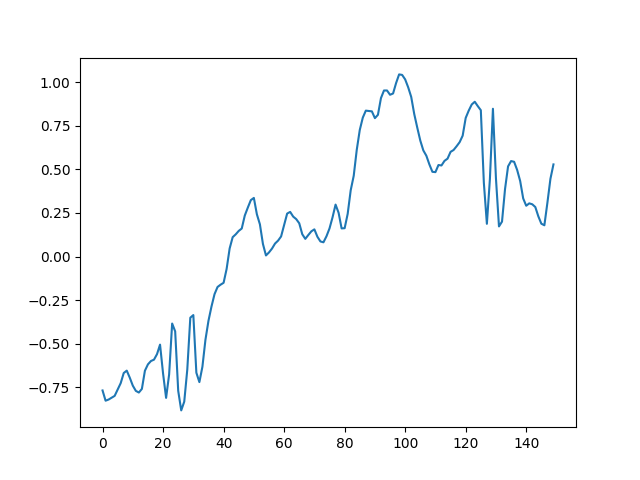
\includegraphics[scale=0.5]{10003csv_axisxpeaks.png}
	\caption{Plot of the x axis samples of training sample 10003.csv}
\end{figure}

\subsection{Average measure between successive peaks}
For each sample I calculated the average of the distances  between the successive peaks of each axis.

\subsection{Magnitude}
The magnitude values for both the time and frequency domains were selected as features (Fig 2, Fig. 3). These were obtained by computing the sum of the square root of the squares of the accelerometer axis data and dividing the sum by the number of acceleration samples in a training sample (150).  

\begin{figure}[h]
	\centering
	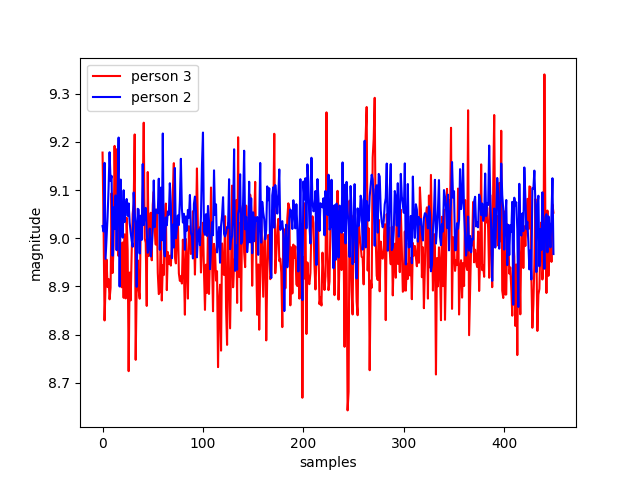
\includegraphics[scale=0.36]{magnitude46_time_dmn.png}
	\caption{Plot of the magnitudes across all 450 training samples for person 2 and 3 (time domain)}
\end{figure}

\begin{figure}[h]
	\centering
	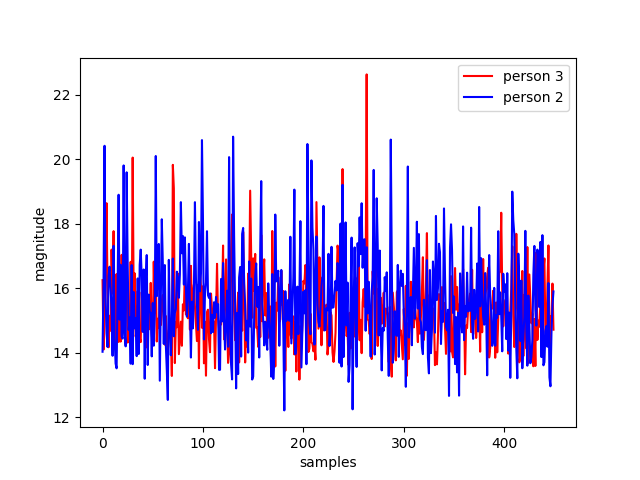
\includegraphics[scale=0.36]{magnitude46_freq_dmn.png}
	\caption{Plot of the magnitudes across all 450 training samples for person 2 and 3 (frequency domain)}
\end{figure}

\subsection{Spectral Centroid}
This measure represents the "center of mass" of the spectrum of each value domain (for each axis). It is computed as the dot product between the axis value vector and its respective FFT vector divided by 150.

\subsection{Average distance from mean}
Totalling a number of six features, this characteristic is computed by taking the average of the absolute values of the differences between each value from an axis and the axis' mean value. 

\section{Models Trained on the Dataset}
My first try was to train the Decision Tree Classifier on an augmented data set with 12 features (mean x,y,z; median x,y,z; cross correlation xy;yz; magnitude (time domain); average distance from mean x;y;z (time domain). I split the data into train and validation samples (validation size of 2000), but unfortunately the accuracy for both the train and validation samples was bad (~76\%). This made me try the Random Forest Classifier, which had better results by a large margin (~0.9±0.1 accuracy on validation samples). My first submission had an accuracy of 0.779 on the test samples provided on the Kaggle competition, which was just below the baseline.

In my second try I gathered more features (everything from the last chapter apart from cross correlation values in the frequency domain) and the results (Table 1), having improved by a relatively large margin, were very close to my third try. I also implemented cross validation (10 fold) to avoid overfitting.

\begin{table}[h]
	\centering
	\caption{10 fold cross validation accuracy scores}
	\label{table1}
	\begin{tabular}{cccc}
		\bottomrule
		\multicolumn{2}{|c|}{\textbf{Random Tree Classifier}} &
		\multicolumn{2}{c|}{\textbf{Decision Tree Classifier}} \\
		\toprule
		\textbf{Fold}& \textbf{Accuracy}& \textbf{Fold}& \textbf{Accuracy} \\
		\midrule
		1 & 0.951 & 1 & 0.864 \\
		2 & 0.938 & 2 & 0.857 \\
		3 & 0.934 & 3 & 0.855 \\
		4 & 0.947 & 4 & 0.876 \\
		5 & 0.938 & 5 & 0.858 \\
		6 & 0.942 & 6 & 0.864 \\
		7 & 0.935 & 7 & 0.86 \\
		8 & 0.938 & 8 & 0.853 \\
		9 & 0.927 & 9 & 0.867 \\
		10 & 0.945 & 10 & 0.863 \\
 		\bottomrule
	\end{tabular}
\end{table}

In my third and final try I decided to do hyperparameter tuning for the Random Tree Classifier, as it had a higher accuracy than the Decision Tree model with the default parameters. For this I created a random grid composed of arrays of:
\begin{itemize}
\item number of estimators: 64, 128,...,2048,
\item maximum features parameter (auto, sqrt, log2),
\item maximum depth (from 10, 20,..., 200), 
\item minimum saples split: 2, 5, 10,
\item minimum saples leaf: 1, 2, 4.
\end{itemize} 

I used this grid with a randomized search and obtained the following parameters: 
\begin{verbatim}
{'n_estimators': 1920, 'min_samples_split': 2,
	'min_samples_leaf': 1, 'max_features': 'sqrt',
	'max_depth': 180, 'bootstrap': False}
\end{verbatim}

Fitting the Random Tree Classifier on the augmented dataset with these parameters slightly incresed the accuracy (by an average of ~4.6\%), as seen in Table 2.

\begin{table}[h]
	\centering
	\caption{10 fold cross validation accuracy scores after hyperparamter tuning}
	\label{table1}
	\begin{tabular}{cc}
		\bottomrule
		\multicolumn{2}{|c|}{\textbf{Random Tree Classifier}} \\
		\toprule
		\textbf{Fold} & \textbf{Accuracy} \\
		\midrule
		1 & 0.937 \\
		2 & 0.954 \\
		3 & 0.948 \\
		4 & 0.937 \\
		5 & 0.938 \\
		6 & 0.966 \\
		7 & 0.941 \\
		8 & 0.943 \\
		9 & 0.94 \\
		10 & 0.938 \\
 		\bottomrule
	\end{tabular}
\end{table}

Below are the confusion matrices (Fig. 4) computed for the two models fit on the full augmented dataset, with a validation set of 2000 samples.

\begin{figure}[hbt!]
	\centering
	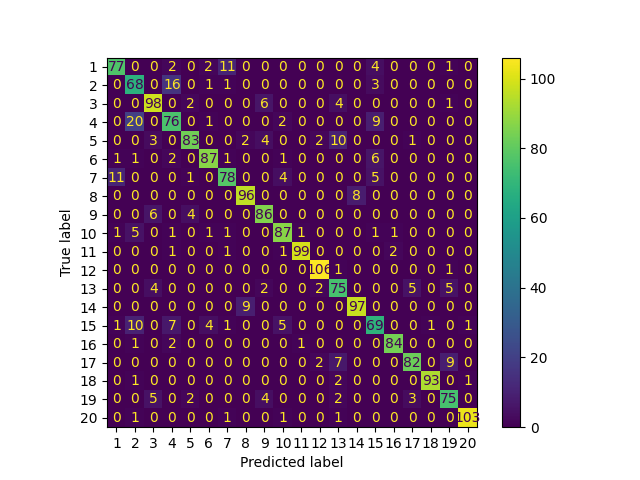
\includegraphics[scale=0.45]{conf_matrix_dt.png}
	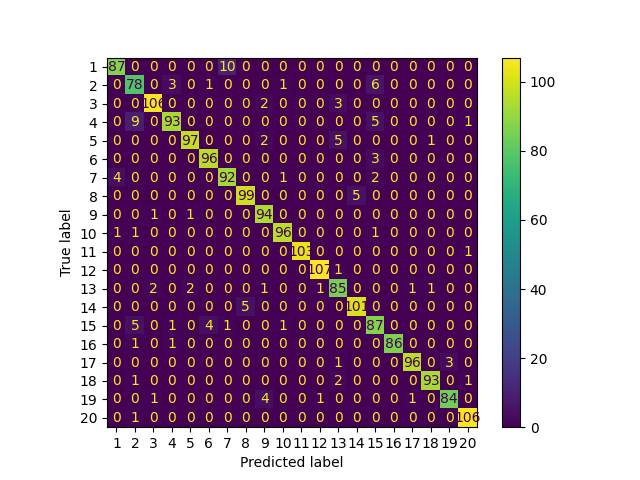
\includegraphics[scale=0.45]{conf_matrix_rfc.png}
	\caption{Decision Tree (left) and Random Forest (right) Confusion Matrices}
\end{figure}

\newpage

\section{Conclusion}
The model that I used to receive the best results was the Random Tree Classifier, which beat the Decision Tree Classifier by a relatively large margin in terms of accuracy. From my point of view, the parts of solving the classification problem which posed the greatest difficulty was exploring and understanding the data and feature engineering. Hyperparameter tuning for the Random Forest, while indeed improving its accuracy, showed diminishing returns for the increased processing time.   

\newpage

\bibliographystyle{IEEEtran}

%\bibliography{template} %-->reference list is on the template.bib file
\begin{thebibliography}{1.7} 
	\bibitem[1]{pandas}\url{https://pandas.pydata.org/}
	\bibitem[2]{findpeaks}\url{https://docs.scipy.org/doc/scipy/reference/generated/scipy.signal.find_peaks.html}
\end{thebibliography}

\end{document}